%!TEX root = main.tex

\clearpage
\appendix

\section{Proof of Theorem~\ref{theo:main}}
\label{app:prooftheo1}

    Let us recall the composite problem of interest. For $\lambda_1, \lambda_2 > 0$ we write the objective functional as
    \begin{equation*}
        \mathcal{J}(\fb, \fh) := \frac{1}{2} \| \bm{y} - (\phib (\fb) + \phih (\fh)) \|_2^2  + \lb \| \fb \|_{\mathcal{B}} + \frac{\lh}{2} \| \fh \|_{\mathcal{H}}^2.
    \end{equation*}
    
    % \begin{proof}
    
    % We define the cost function 
    % \begin{equation*}
    %     \mathcal{J}(\fb, \fh)
    %     =\| \bm{y} - (\phib (\fb) + \phih (\fh)) \|_2^2  + \lb \| \fb \|_{\mathcal{B}} + \lh \| \fh \|_{\mathcal{H}}^2.
    % \end{equation*}
    Assume first that $\fb$ is fixed and consider the optimization problem $\inf_{s_2 \in \mathcal{H}} \mathcal{J}(\fb, \fh)$. It is clearly equivalent to
    \begin{equation*}
        % \mathcal{U} ( (\bm{y} - \phib(\fb)), \phih, \lh) =
        \underset{\fh \in \mathcal{H}}{\arg\min}  \quad \frac{1}{2} \| (\bm{y} - \phib(\fb)) - \phih(\fh) \|_2^2 + \frac{\lh}{2} \| \fh \|_{\mathcal{H}}^2,
    \end{equation*}
    whose unique solution according to Proposition~\ref{prop:hilbertRT}, depends on $\fb$ and is given by
    \begin{equation}
        \label{eq:hatfwithfb}
        \widehat{s}_{2, \fb} =\phih^* ( \phih \phih^* + \lh \mathbf{I}_L)^{-1} ( \bm{y} - \phih(\fb) ). 
    \end{equation}
    Using the latter relation, we therefore deduce that $(\hfb,\hfh) \in \mathcal{W} (\lb,\lh)$ if and only if  
    \begin{align}
        \hfh &= \widehat{s}_{2,\hfb} = \phih^* ( \phih \phih^* + \lh \mathbf{I}_L)^{-1} ( \bm{y} - \phib(\hfb) ) , \quad \text{and} \label{eq:findmethishfh}\\
        \hfb &\in\underset{\fb \in \mathcal{B}}{\arg\min}  \quad \mathcal{J}(\fb, \widehat{s}_{2, \fb}) \label{eq:newhproblem}
    \end{align}
    % where
    % \begin{equation}
    % \label{eq:newcostfb}
    %     \mathcal{J}(\fb) = \| \bm{y} - \phih( \widehat{f}_{2, \fb} ) -  \phib (\fb) \|_2^2 + \lb \| \fb \|_{\mathcal{B}} + \lh \|  \widehat{f}_{2, \fb}\|_{\mathcal{H}}^2.
    % \end{equation}

    Replacing $\widehat{s}_{2, \fb}$ with its expression~\eqref{eq:hatfwithfb}, we observe that
    \begin{align}
        \| \bm{y} - \phih( \widehat{s}_{2, \fb} ) - \phib (\fb) \|_2^2 &= 
        \| (\mathbf{I}_L - \phih \phih^*( \phih \phih^* + \lh \mathbf{I}_L)^{-1}) ( \bm{y} - \phib (\fb) ) \|_2^2 \nonumber  \\
        &= \lh^2 \| ( \phih\phih^* + \lh \mathbf{I}_L)^{-1} (\bm{y} - \phib(\fb) ) \|_2^2 \label{eq:firstinterm}
    \end{align}
    simply using that $\mathbf{I}_L - \phih\phih^*( \phih\phih^* + \lh \mathbf{I}_L)^{-1} = \lh ( \phih\phih^* + \lh \mathbf{I}_L)^{-1}$. 

    Moreover, using again \eqref{eq:hatfwithfb} and the fact that $\phih\phih^* ( \phih\phih^* + \lh \mathbf{I}_L)^{-1} = \mathbf{I}_L - \lh ( \phih\phih^* + \lh \mathbf{I}_L)^{-1}$, the Hilbert penalty term rewrites as
    \begin{align}
        \|  \widehat{s}_{2, \fb}\|_{\mathcal{H}}^2 
        &=
        \langle \phih^* ( \phih\phih^* + \lh \mathbf{I}_L)^{-1} ( \bm{y} - \phih(\fb) ) , \phih^* ( \phih\phih^* + \lh \mathbf{I}_L)^{-1} ( \bm{y} -  \phib (\fb) ) \rangle_{\mathcal{H}} \nonumber \\
        &=
        \langle ( \phih\phih^* + \lh \mathbf{I}_L)^{-1} ( \bm{y} - \phib(\fb) ) ,  \phih \phih^* ( \phih \phih^* + \lh \mathbf{I}_L)^{-1} ( \bm{y} - \phib(\fb) ) \rangle \nonumber \\
        &= 
        \langle ( \phih \phih^* + \lh \mathbf{I}_L)^{-1} ( \bm{y} - \phib(\fb) ) ,  ( \bm{y} - \phib(\fb) ) \rangle - \lh \|( \phih \phih^* + \lh^2 \mathbf{I}_L)^{-1} ( \bm{y} - \phib(\fb) ) \|_2^2.   \label{eq:secondinterm} 
    \end{align}
    Finally, plugging the relations \eqref{eq:firstinterm} and \eqref{eq:secondinterm} together,  the cost functional $\mathcal{J}(\fb, \widehat{f}_{2, f_1})$ in \eqref{eq:newhproblem} simplifies as
    \begin{align*}
        \mathcal{J}(\fb, \widehat{s}_{2, \fb}) &=  \frac{\lh}{2} \langle ( \phih \phih^* + \lh \mathbf{I}_L)^{-1} ( \bm{y} - \phib(\fb) ) ,  ( \bm{y} - \phib(\fb) ) \rangle + \lb \|\fb\|_{\mathcal{B}} \nonumber \\
        &= \frac{\lh}{2} \| ( \phih \phih^* + \lh \mathbf{I}_L)^{-\frac{1}{2}} (\bm{y} - \phib(\fb) ) \|_2^2 + \lb \|\fb\|_{\mathcal{B}} \\
        &= \frac{1}{2}\| \mathbf{M}_{\lh}^{-\frac{1}{2}} (\bm{y} - \phib(\fb) ) \|_2^2 + \lb \|\fb\|_{\mathcal{B}}.
    \end{align*}
    This shows the first relation~\eqref{eq:banachpart}. According to Proposition~\ref{prop:banachRT}, this optimization problem admits a solution and therefore the solution set $\mathcal{W} (\lb,\lh)$ is non-empty. 

    Proposition~\ref{prop:banachRT} also implies that all the $\hfb$ solution of \eqref{eq:newhproblem} share the same measurement vector $\mathbf{M}_{\lh}^{-\frac{1}{2}} \phib (\hfb)$. Hence $\bm{w} = \phib(\hfb) \in \R^L$ is the common measurement vector of the Banach components $\hfb$ of the solutions $(\hfb , \hfh) \in \mathcal{W} (\lb,\lh)$, which proves \eqref{eq:hilbertpart}.

    % vector $\bm{w} (\mathbf{M}_{\lh}^{-\frac{1}{2}} \bm{y}, \mathbf{M}_{\lh}^{-\frac{1}{2}} \phib,\lb / \lh)$ which is the common measurements of the Banach components $\hfb$ of the solutions $(\hfb , \hfh) \in \mathcal{W} (\bm{y}, \bm{\Phi} ,\lb,\lh)$. In particular, $\bm{w} (\mathbf{M}_{\lh}^{-\frac{1}{2}} \bm{y}, \mathbf{M}_{\lh}^{-\frac{1}{2}} \phib,\lb / \lh) = \phib ( \hfb)$ in \eqref{eq:findmethishfh} and \eqref{eq:hilbertpart} is proved.
    
    %\end{proof}

\clearpage
\section{Discretization of the Banach Decoupled Subproblem}
    \label{app:discretization}
        Remember that we want to solve the following problem
        $$s_1^* \in \underset{ s_1\in\mx}{\arg\min} \quad \mathcal{J}_{\mathbf{M}}(s_1)$$
        with
        $$\mathcal{J}_{\mathbf{M}}(s_1)= \|\mathbf{M}_{\lh}^{-\frac{1}{2}} ( \bm{y} - \phib(s_1)  ) \|_2^2  + \lb \| s_1 \|_{\mathcal{M}}.$$
        We know that there exist sparse solutions, which takes the form $s_1^* = \sum_k \alpha_k \delta_{z_k}$ for $z_k\in\mathcal{X}$.

        Let us introduce the $d$-dimensional fine grid $G_J$ of size $J^d$ defined as
        \begin{equation*}
            G_J = \left\{ \left(\frac{j_1}{J-1}, \dots, \frac{j_d}{J-1} \right) : 0 \leq  j_1, \dots, j_d \leq J-1 \right\}.
        \end{equation*}
        To maintain super-resolution with respect to the sampled data, the grid size $J$ is chosen much larger than the measurements grid size $K$. We define the space of Radon measures with support on this grid as
        \begin{equation*}
            V^1_J = \left\{ s \in \mathcal{M}(\mathbb{R}) : \mathrm{Supp}(s) \in G_J \right\}.
        \end{equation*}
        We then approximate the decoupled minimization \eqref{eq:deconv-banachpart} with
        \begin{equation}
            \label{eq:discrete-banach}
            s_{1, J}^* \in \underset{ s_1\in V^1_J}{\arg\min} \quad \mathcal{J}_\mathbf{M}(s_1)
        \end{equation}
        For any $s \in V^1_J$, we can write $s = \sum_j \alpha_j \delta (\cdot - z_j) $, hence
        $$
        \bm{\Phi}(s)[\ell] = \sum_j \alpha_j g(x_{\ell} - z_j)
        $$
        so that we can express 
        $$
        \bm{\Phi}(s) = \mathbf{H}\bm{a}.
        $$
        The matrix $\mathbf{H} \in \R^{L \times J^d}$ performs the convolution between the weights $\bm{a}$ and the measurement kernel $g$ sampled on the reconstruction grid and shifted to the sampling locations $x_{\ell}$. 
        % In the simple case $d=1$, we obtain $\mathbf{H}[\ell, j] = g(x_{\ell} - z_j)$ for $1 \leq \ell \leq L $ and $1 \leq j \leq J$.
        
        
        Problem \eqref{eq:discrete-banach} is then equivalent to the finite-dimensional LASSO problem
        \begin{equation*}
            \underset{ \bm{a} \in \mathbb{R}^{J^d}}{\arg\min} \quad ( \bm{y} - \mathbf{H}\bm{a}  )^T \mathbf{M}_{\lh}^{-1} ( \bm{y} - \mathbf{H}\bm{a}  )  + \lb \| \bm{a} \|_{1}.
        \end{equation*}    

\clearpage

\section{Error on the Reconstruction of the Background}
    \label{app:errorbg}

    The $\mathrm{RE}_2$ error on the background is reported in the following table. The best values are obtained with a certain trade-off between the two regularization parameters.  

    \begin{table}[h]
        \centering
        \begin{tabular}{l|rrrr}
            \toprule
             & \multicolumn{4}{c}{$\lambda_2$} \\
            \cmidrule(lr){2-5}
            $\alpha_1$ & 0.80 & 4.00 & 8.00 & 40.00 \\
            \midrule
            0.02 & \textbf{0.049} & 0.484 & 0.697 & 0.907 \\
            0.05 & 0.130 & 0.082 & 0.309 & 0.778 \\
            0.10 & 0.234 & 0.156 & 0.096 & 0.578 \\
            0.15 & 0.311 & 0.243 & 0.165 & 0.409 \\
            \bottomrule
        \end{tabular}
        \caption{Relative $\ell_2$-norm error on the background components \label{tab:rl2-bg}}
    \end{table}

    \vfill

\section{Composite Reconstructions}
    \label{app:reconstructions}

    % \vfill

    Figure~\ref{fig:simple:fg-merged} displays the various reconstructions of the foreground component when varying the regularization parameters. Figure~\ref{fig:simple:bg} does the same for the background component. Note that the value of $\lb$ is not provided in these plots, only the coefficient $\alpha = \lambda_1 / \lambda_{1, \mathrm{max}}$. This reparametrization somehow interleaves the value of the parameters, indeed $\lambda_1$ strongly depends on the value of $\lambda_2$ (that is, in each column, $\lambda_1$ varies across the rows). However, this choice seems relevant as it almost decouple the choice of the parameters. Each column in the foreground reconstructions display similar sparsity characteristics. The choice of $\lambda_2$ mostly has impact on the recovered background.

    \vfill

    % trim={left bottom right top},clip
    \begin{figure}[p]
        % \centering
        % 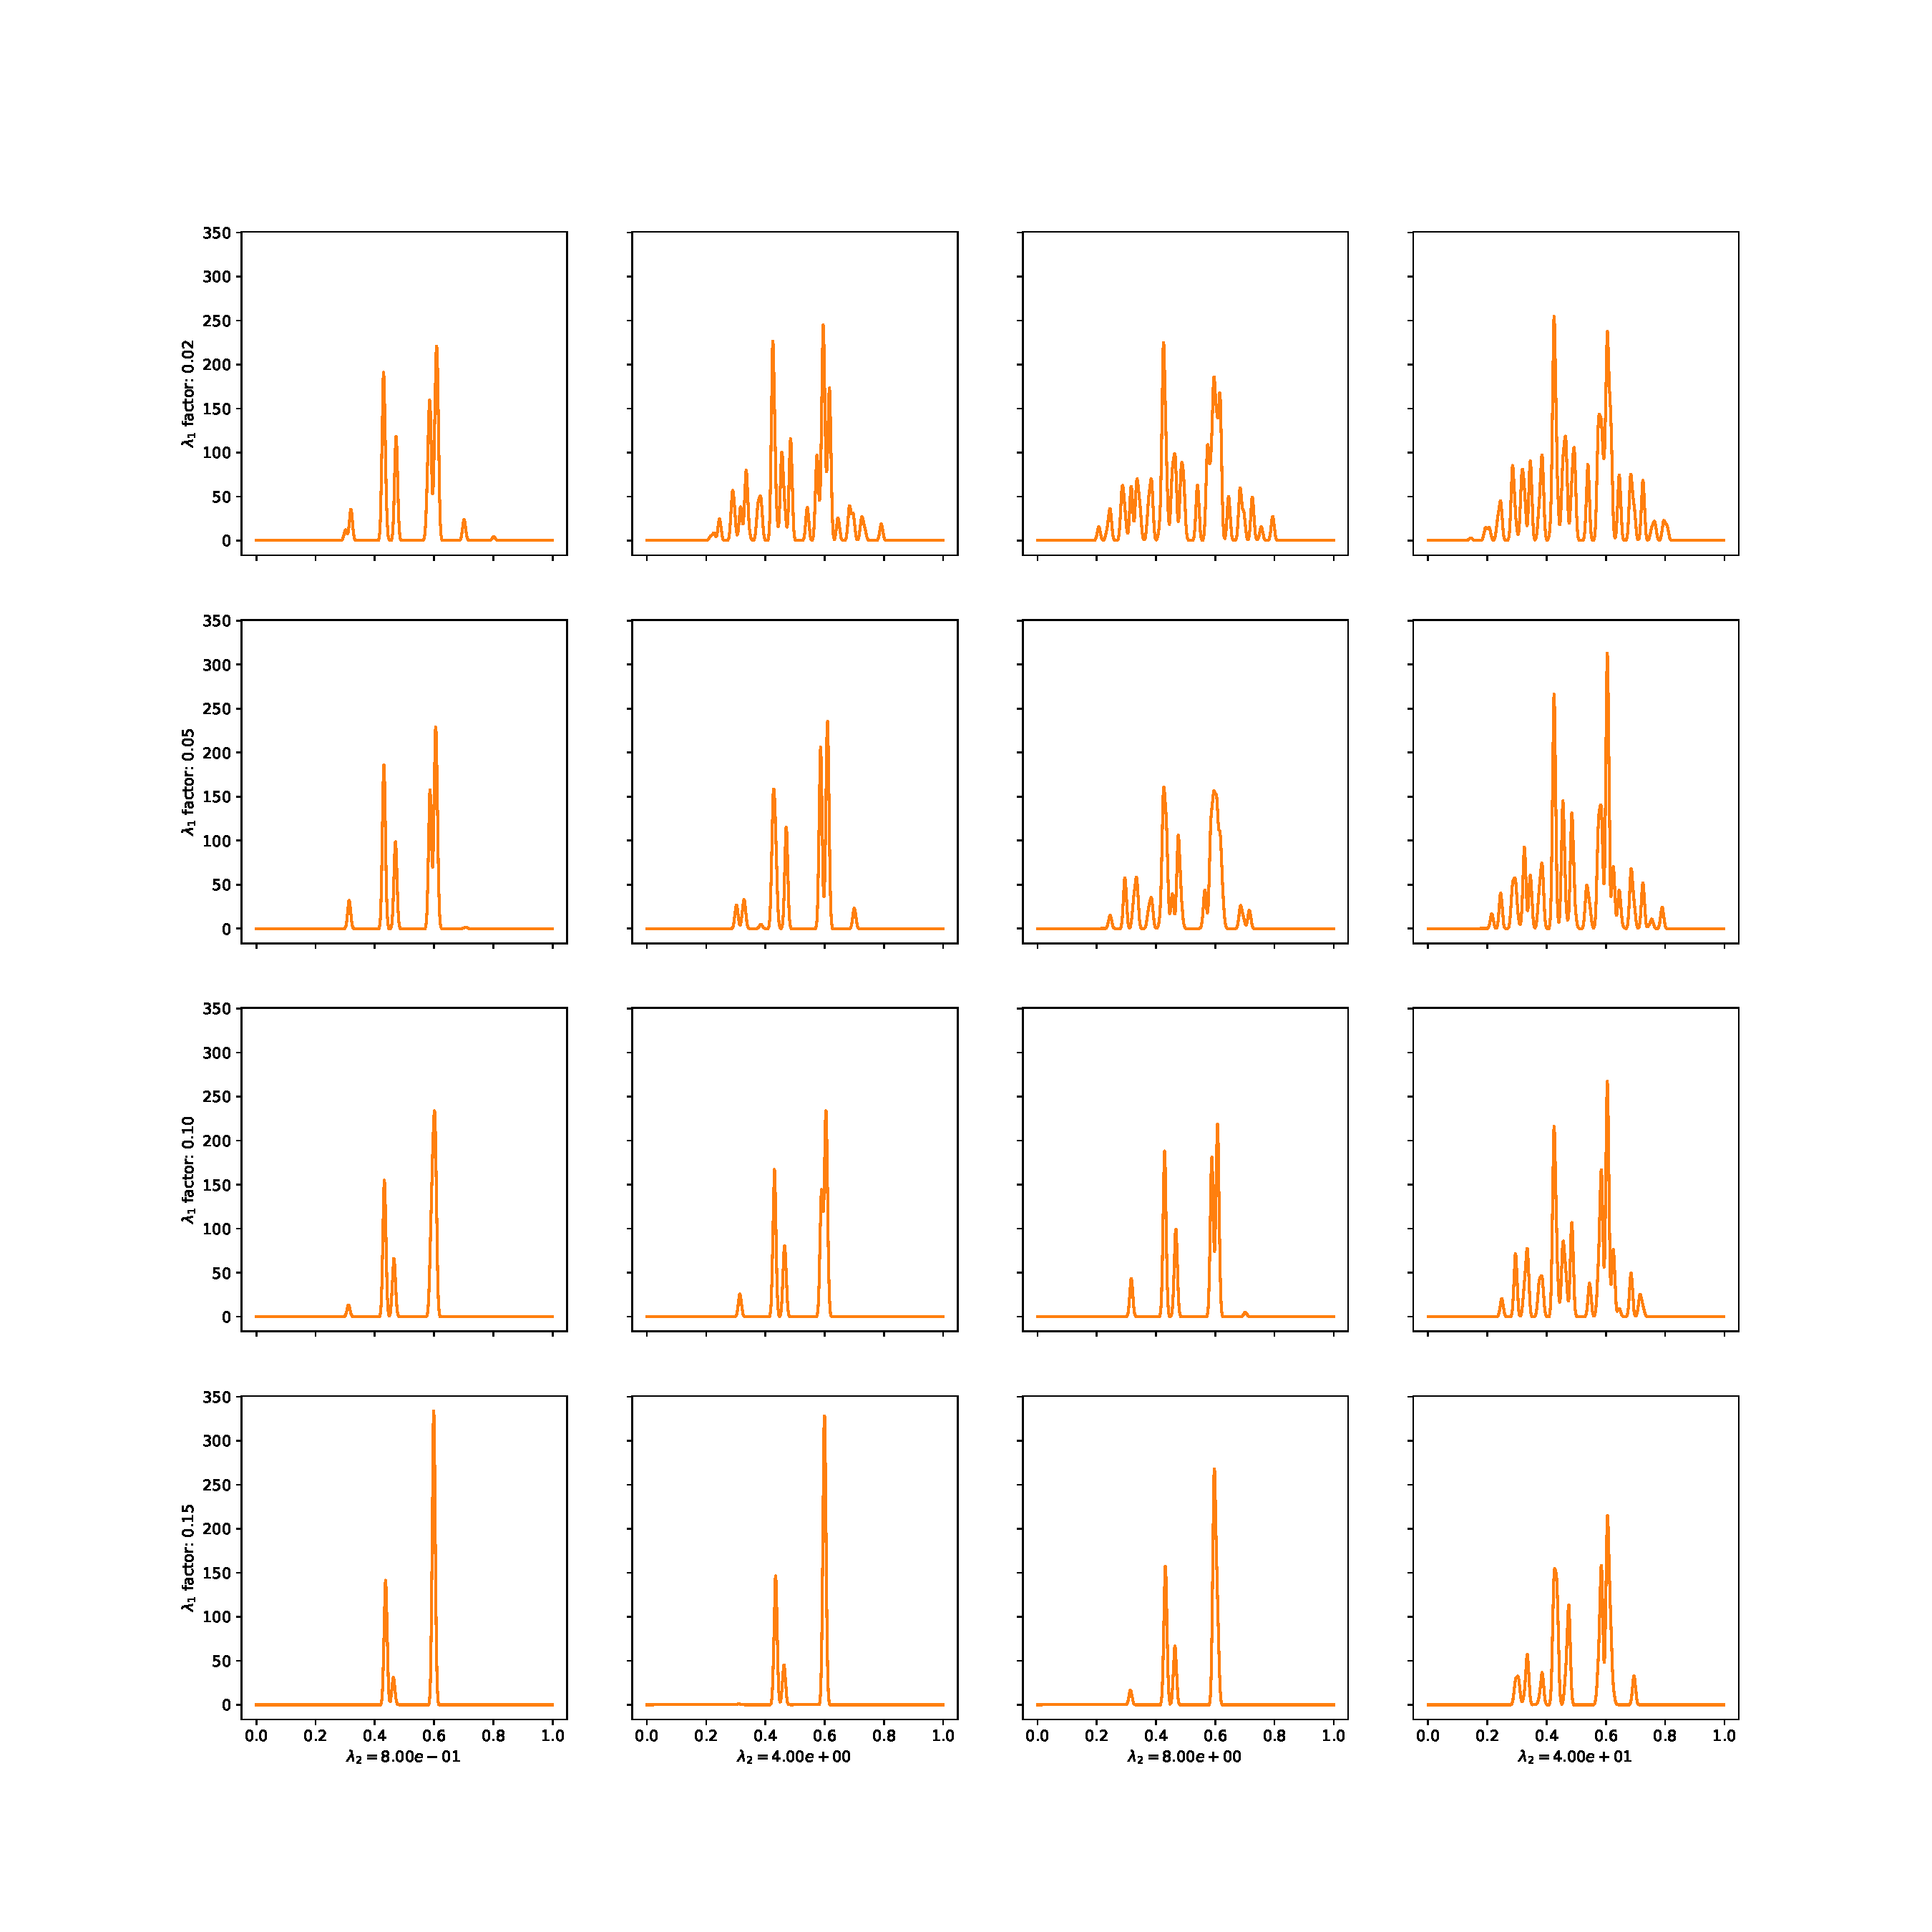
\includegraphics[width=1.2\linewidth]{figures/simple_reco/foreground_merged.pdf}
        \makebox[\textwidth][c]{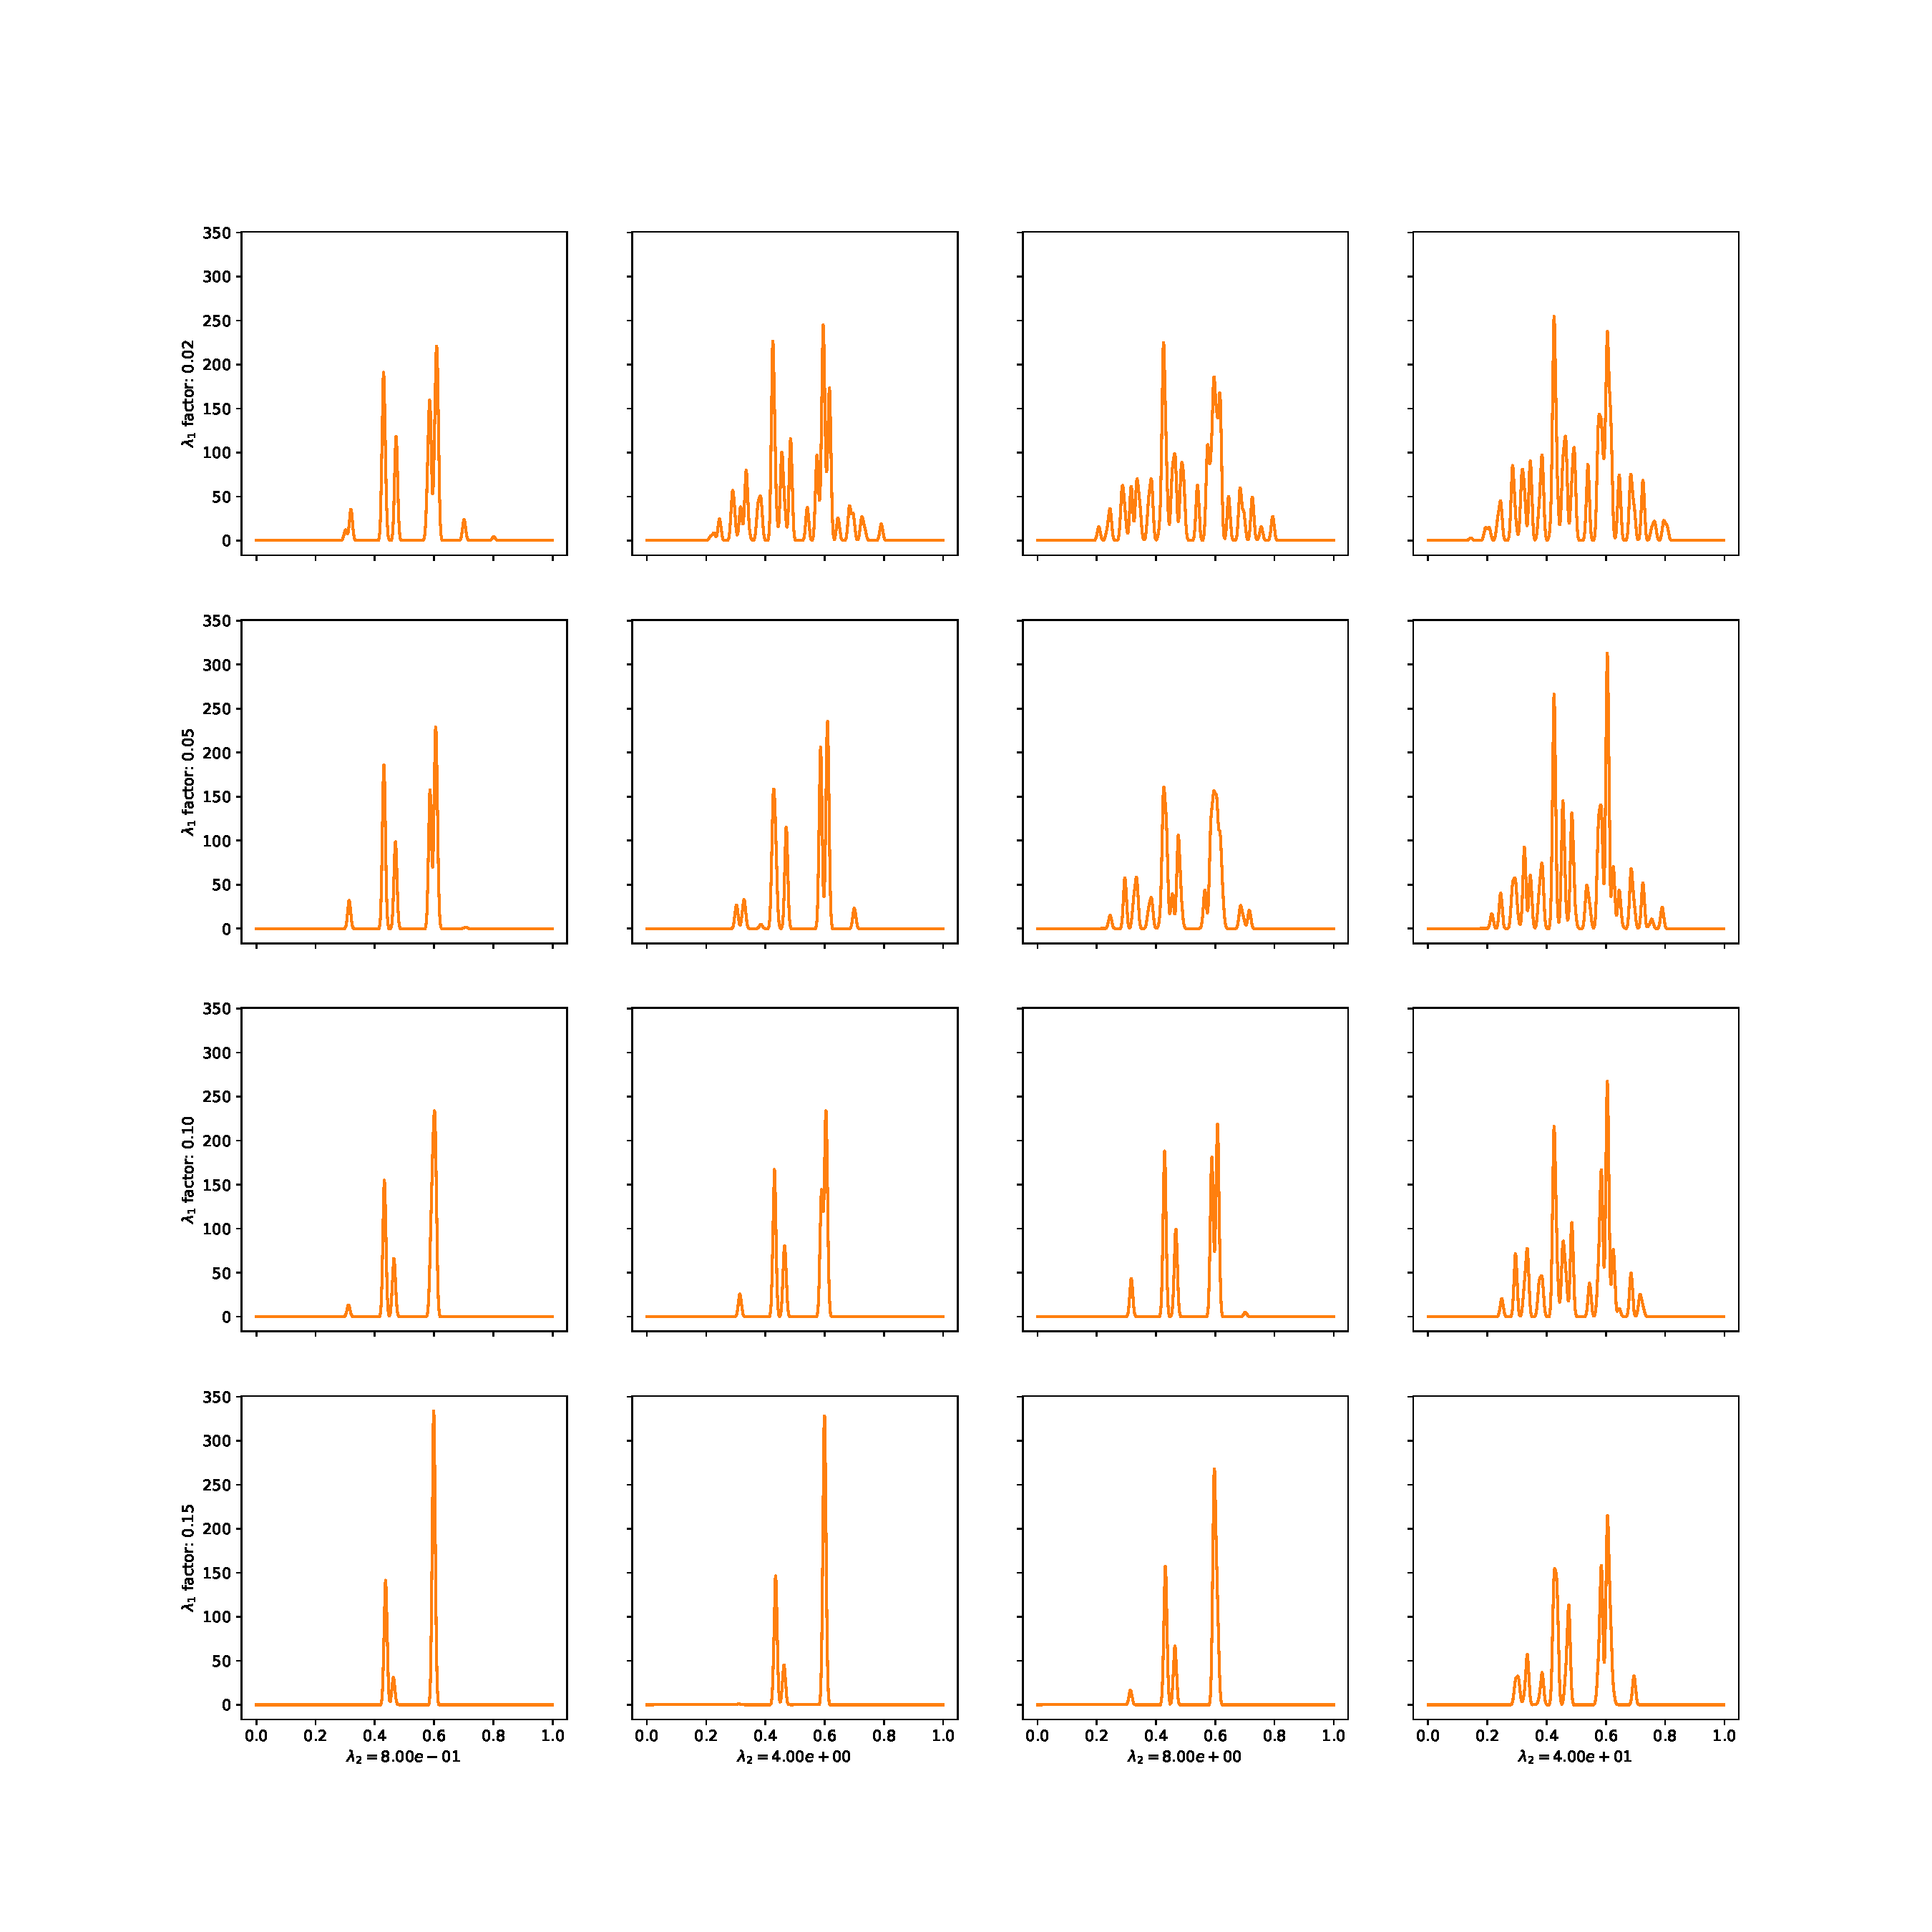
\includegraphics[width=1.1\linewidth, trim=2cm 2.5cm 2cm 3.7cm, clip]{figures/simple_reco/foreground_merged.pdf}}
        \caption{Recovered foreground after convolution with the representation kernel. \textit{Rows :} Increasing value of $\lambda_2$ from top to bottom. \textit{Columns :} Increasing factor $\alpha$ from left to right.}
        \label{fig:simple:fg-merged}        
    \end{figure}

    % \vfill

    \begin{figure}[p]
        \makebox[\textwidth][c]{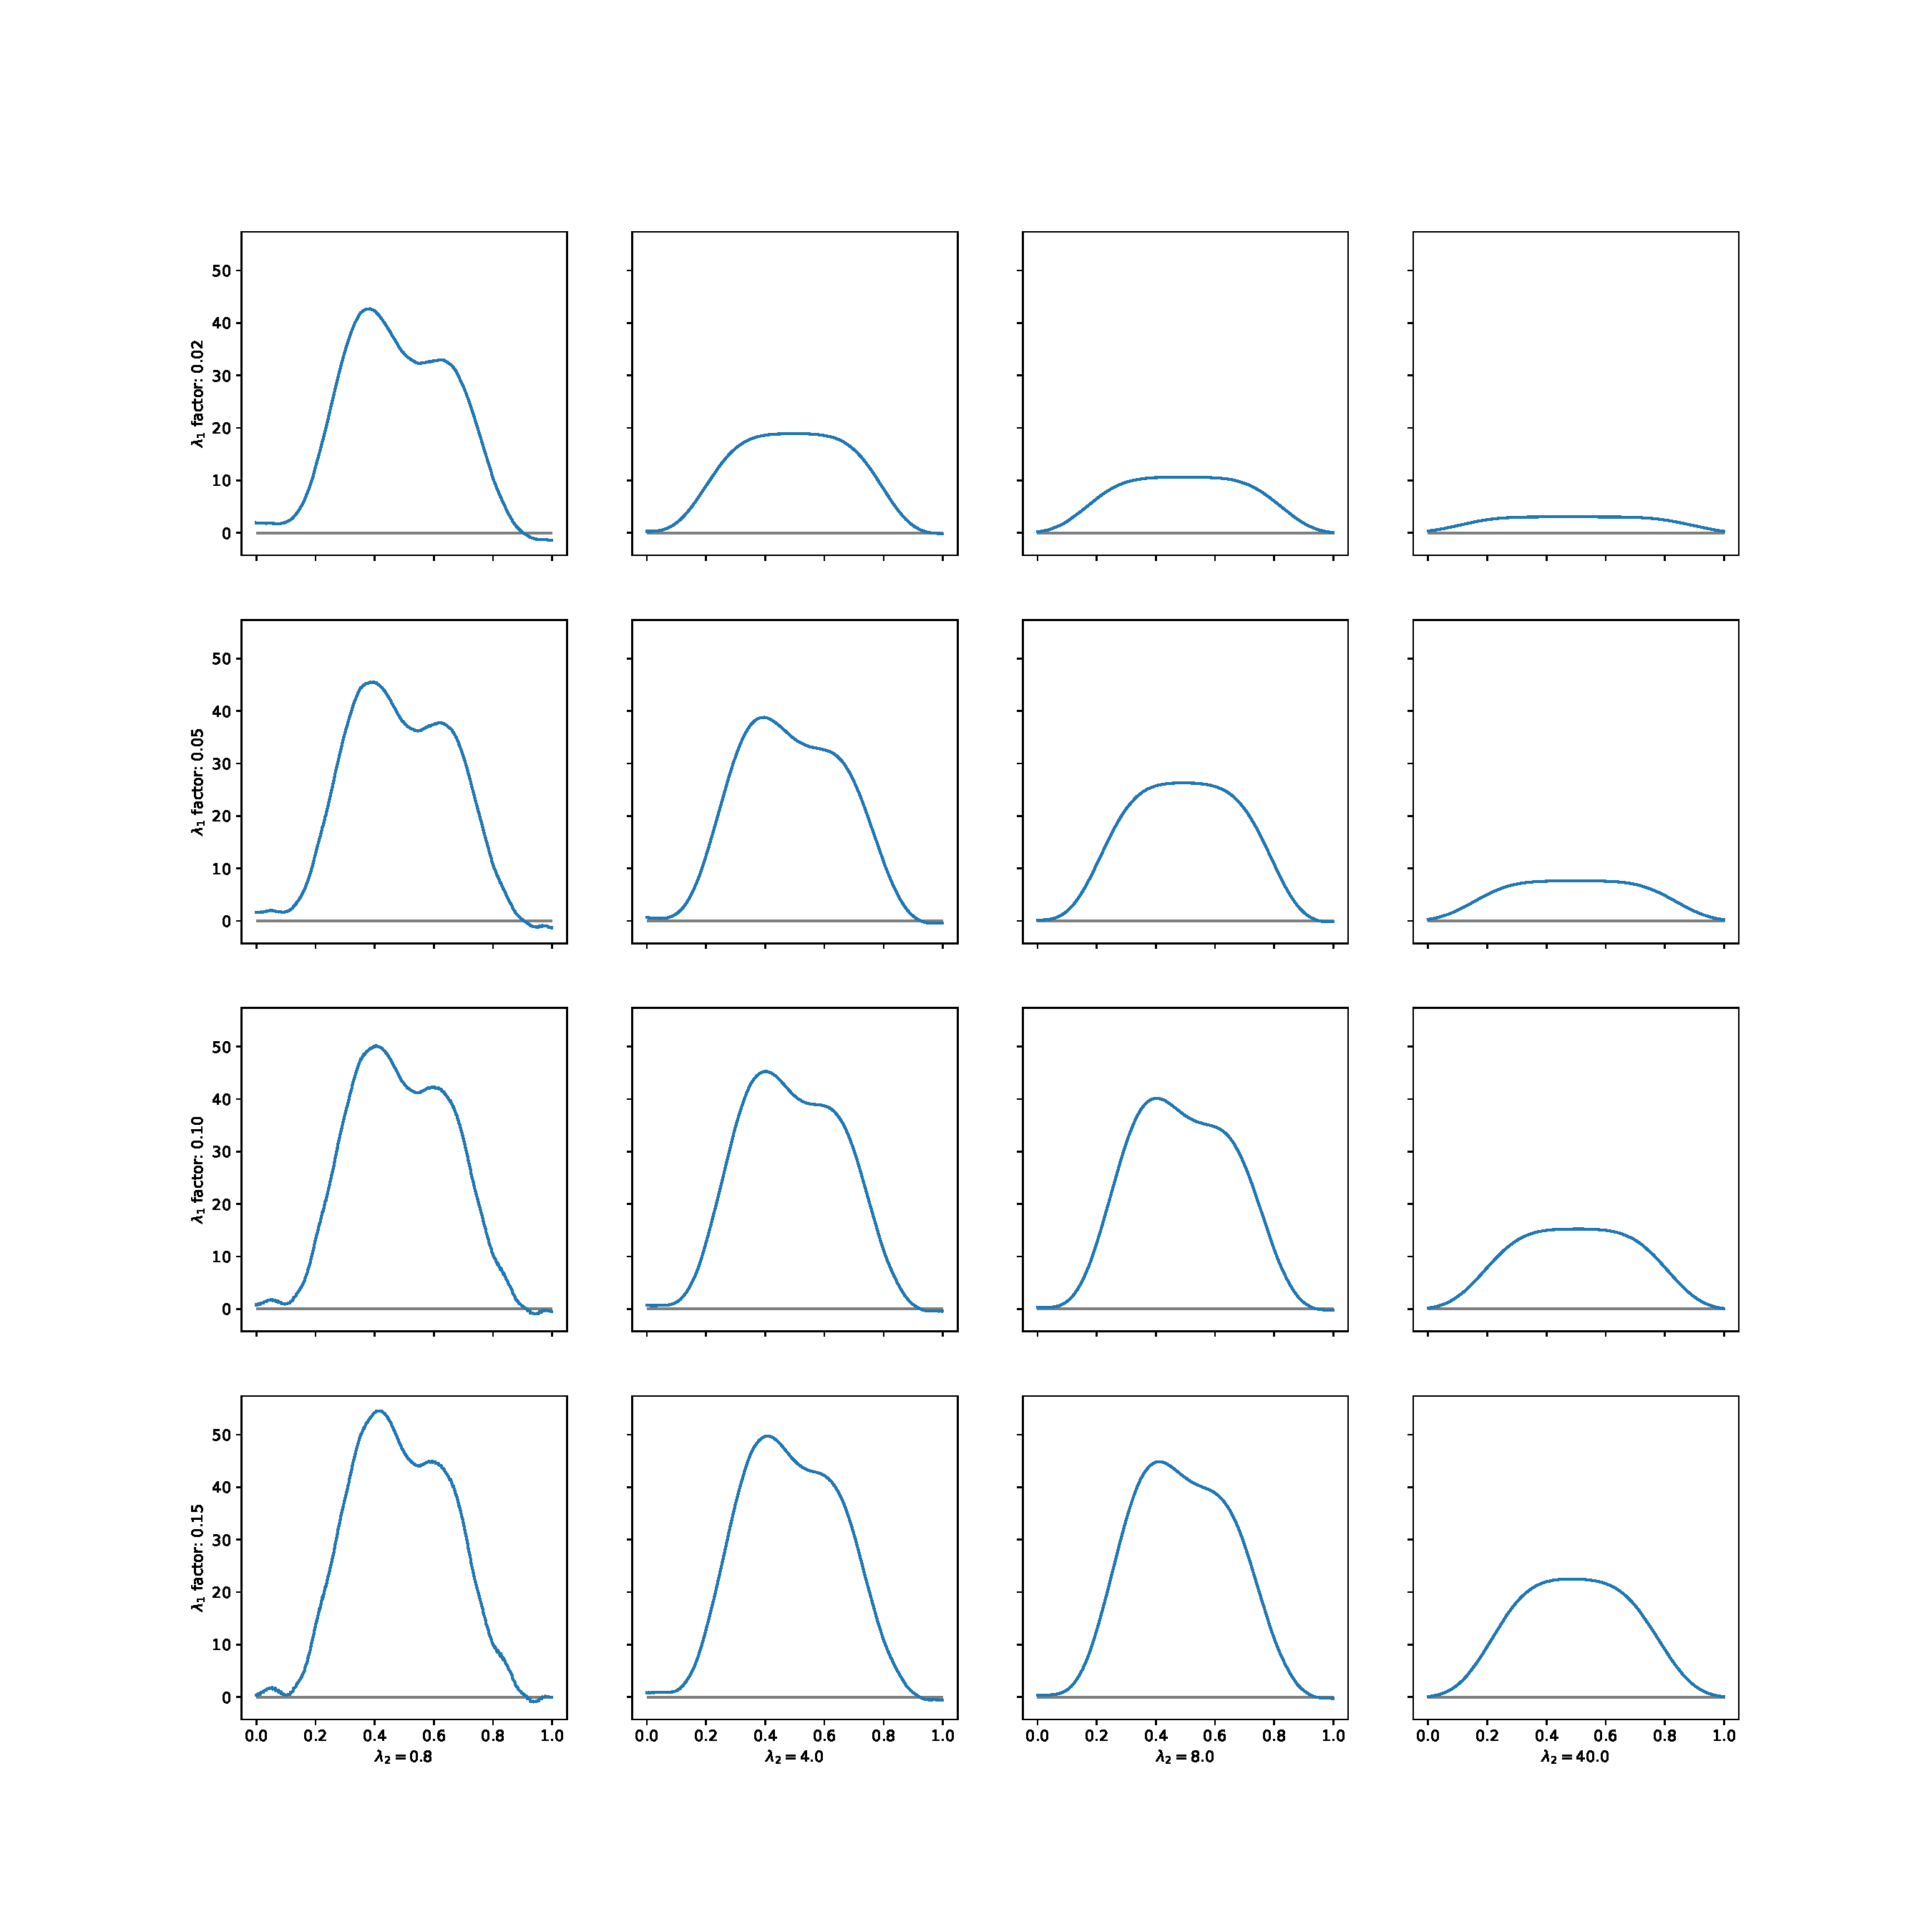
\includegraphics[width=1.1\linewidth, trim=2cm 2.5cm 2cm 3.7cm, clip]{figures/simple_reco/backgrounds.pdf}}
        \caption{Recovered background components, with the same value of regularization parameters as in figure~\ref{fig:simple:fg-merged}.}
        \label{fig:simple:bg}        
    \end{figure}


\clearpage
\section{Calculation for the Experiments}
    \label{app:calculation}

    \subsection{Computation of \texorpdfstring{$M_{\lh}$}{M lambda 2}}

    Using the definition of the PSF $g$ in section~\ref{sec:application}, we derive the expression of the matrix $\mathbf{M}_{\lambda_2}$ defined in equation~\eqref{eq:def-Mphi}. For $1\leq k, \ell \leq L$, we have:
    \begin{equation*}
        \mathbf{M}_{\lh}[k, \ell] = \frac{1}{\lh} \left( \langle \phi_k , \phi_\ell \rangle_{\mathcal{H}} + \lh \delta[k - \ell] \right)
    \end{equation*}
    Let us compute the inner product between the functionals $\phi$
    \begin{equation*}
        \begin{aligned}
            \langle \phi_k , \phi_\ell \rangle_{\mathcal{H}} &= \int_\mathcal{X} g(x_k - t) g(x_\ell - t) \mathrm{d}t \\
                &= \int_\mathcal{X} g(- t) g(x_\ell - x_k - t) \mathrm{d}t \\
                &= \int_\mathcal{X} g(t) g(x_\ell - t) \mathrm{d}t \\
                &=  (g * g)(x_\ell - x_k)
        \end{aligned}
    \end{equation*}
    using the symmetry of the kernel $g$ between lines 2 and 3.
    We finally obtain the expression
    \begin{equation*}
        \label{eq:mlambda-1d}
        \mathbf{M}_{\lambda_2}[k, \ell] = \frac{1}{\lh} \left( (g * g)(x_\ell - x_k) + \lh \delta [k - \ell] \right) .
    \end{equation*}

    \subsection{Scaling of \texorpdfstring{$\lh$}{lambda 2}}
    From equation~\eqref{eq:def-Mphi}, the matrix $\mathbf{M}_{\lambda_2}$ can be written as
    \begin{equation}
        \label{eq:mlambda2}
        \mathbf{M}_{\lh} = \mathbf{I}_L +  \frac{1}{\lh}\phih\phih^*
    \end{equation}
    For any vector $\mathbf{h} \in \R^L$, we have
    \begin{align*}
        \forall 1 \leq k \leq L, \quad \left(\phih\phih^*\mathbf{h}\right)[k] &= \sum_\ell \langle \phi_k , \phi_\ell \rangle_{\mathcal{H}} h_\ell \\
            &= \sum_\ell (g * g)(x_\ell - x_k) h_\ell \\
            &= \sum_\ell u_{k - \ell} h_\ell,
    \end{align*}
    with $u_i = (g * g)(x_i)$ for $ \leq i \leq L$. Assuming the support of $\mathbf{h}$ is concentrated in the center of the vector and there is no information near the borders, $\phih\phih^*\mathbf{h}$ can be seen as a convolution between $\mathbf{h}$ and $\mathbf{u}$.

    It is possible to prove that the Lipschitz constant of the operator $\phih\phih^* \in \R^{L \times L}$, which is its maximum singular value, is bounded by $\sqrt{L} \norm{\mathbf{u}}$. Using that $\norm{g*g}_2 = 1$, we can approximate $\norm{\mathbf{u}}_2 \approx \sqrt{L}$ using Riemann sum. Hence, we approximate the maximum singular value of $\phih\phih^*$ with $L$.

    To maintain the term $\frac{1}{\lh} \phih\phih^*$ of the same order as $\mathbf{I}_L$ in $\eqref{eq:mlambda2}$, we set $\lh$ as a ratio of $L$ and we obtain our proposed scaling rule $\lh = \alpha_2 L$.
    


% %%%%%%%%%%%%%%%%%%%%%%%%%%%%%%%%%%%%%%%%%%%%%%
% %%%%%%   FOURRETOUT
% %%%%%%%%%%%%%%%%%%%%%%%%%%%%%%%%%%%%%%%%%%%%%%
% \clearpage    
% \section{Fourretout}

%     \begin{itemize}

%         \item Once we have recognized this fact, we can reuse all the known results for the lasso and apply them in this setting. For instance, uniqueness result for the lasso~\cite{tibshirani2013lasso} or the generalized lasso (if we consider non-invertible operators)~\cite{ali2019generalized} apply to the subproblem. For instance, for large class of sensing matrices $\mathrm{A}$, the transformed $\mathrm{A}$ also has good properties and therefore uniqueness occurs almost surely.
%         \item Same idea: with Fourier measurements and $\Lop_1$ elliptic, if I can include non-invertible operators, I deduce uniqueness results.
        
%         \item Do I do matrices also?
        
%     \end{itemize}

%     \begin{itemize}
%         \item The optimization problem \eqref{eq:hilbertargmin} admits a unique solution given by
%         \begin{equation}
%             \hfh = \Lop^{-1}\Lop^{-1*} \bm{\Phi}^* \left( \bm{\Phi} \Lop^{-1} \Lop^{-1*} \bm{\Phi}^* + \lambda_2 \mathbf{I}_L\right)^{-1} \bm{y}. 
%         \end{equation}
%         \item The optimization problem \eqref{eq:banachargmin} admits at least, and possibly more than, one solution. Moreover, all the solutions share the same measurement vector in the sense that there exists $\bm{y}_{\lambda,\bm{\Phi},\Lop} \in \R^L$ such that 
%         \begin{equation}
%            \forall \hfb \in \mathcal{V}_{\lambda} (\bm{y}, \bm{\Phi} ,\Lop), \quad  \bm{\Phi}(\hfb)  = \bm{y}_{\lambda,\bm{\Phi},\Lop}. 
%         \end{equation}
%     \end{itemize}


%         Fix $\bm{y}$ $\bm{\Phi}$ $\Lop_{\mathcal{B}}$ $\Lop_{\mathcal{H}}$ $\lb$ $\lh$ and set
%     \begin{align}
%         \mathcal{W}_{\lb,\lh} (\bm{y}, \bm{\Phi} ,\Lop_{\mathcal{B}}, \Lop_{\mathcal{H}}) &= \underset{(\fb,\fh) \in \mathcal{B} \times \mathcal{H}}{\arg\min} \| \bm{y} - (\phib (\fb) + \phih (\fh)) \|_2^2  + \lb \| \fb \|_{\mathcal{B}} + \lh \| \fh \|_{\mathcal{H}}^2. 
%     \end{align}    



%     Our main result consists in showing a strong connection between the composite optimization task \eqref{eq:compoargmin} and the two subproblems \eqref{eq:hilbertargmin} and \eqref{eq:banachargmin}. 


%     An inverse problem can be described as follow. We aim at recovering an unknown signal (vector, sequence, function, etc.) from the knowledge of possibly corrupted partial observations. Imagine for instance that you aim at reconstructing an unknown vector $\bm{x}_0 \in \R^N$ from an observation vector $\bm{y} = \mathrm{A} \bm{x}_0 + \epsilon \in \R^M$ where $\mathrm{A} \in \R^{N\times M}$ is a (known) sensing matrix and $\epsilon \in \R^M$ is an i.i.d. Gaussian noise. We assume moreover that $M < N$ such that the system is underdetermined. 

%     The reconstruction task is classically formulated as an optimization problem where the indetermination is overcome by the addition of regularization functional. This leads to optimization problems of the form
%     \begin{equation}
%         \min_{\bm{x}\in \R^N} \| \bm{y} - \mathrm{A} \bm{x} \|_2^2 + \lambda \mathcal{R}( \bm{x} ),
%     \end{equation}
%     where $\mathrm{R}$ is a convex regularization functional which makes the problem well-posed (see below) and $\lambda > 0$ is a parameter balancing the importance of the data-fidelity term $\| \bm{y} - \mathrm{A} \bm{x} \|_2^2$ and the regularization $\mathcal{R}( \bm{x} )$. 

%     Typical choices for the regularization include:
%     \begin{itemize}
%         \item \textbf{Tychonov regularization:} $\mathcal{R}(\bm{x}) = \| \bm{x} \|_2^2$.
        
%         \item \textbf{Sparsity-promoting regularization:}$\mathcal{R}(\bm{x}) = \| \bm{x} \|_1$. In that case, \eqref{eq:} is the well-known LASSO, which is known to promote sparsity and has been extensively studied~\cite{tibshirani1996regression}. In particular, there exists a solution $\widehat{x} \in \R^N$ which is $M$-sparse~\cite{gupta2018continuous}. 
%     \end{itemize}